\documentclass[]{article}
\usepackage{lmodern}
\usepackage{amssymb,amsmath}
\usepackage{ifxetex,ifluatex}
\usepackage{fixltx2e} % provides \textsubscript
\ifnum 0\ifxetex 1\fi\ifluatex 1\fi=0 % if pdftex
  \usepackage[T1]{fontenc}
  \usepackage[utf8]{inputenc}
\else % if luatex or xelatex
  \ifxetex
    \usepackage{mathspec}
  \else
    \usepackage{fontspec}
  \fi
  \defaultfontfeatures{Ligatures=TeX,Scale=MatchLowercase}
\fi
% use upquote if available, for straight quotes in verbatim environments
\IfFileExists{upquote.sty}{\usepackage{upquote}}{}
% use microtype if available
\IfFileExists{microtype.sty}{%
\usepackage{microtype}
\UseMicrotypeSet[protrusion]{basicmath} % disable protrusion for tt fonts
}{}
\usepackage[margin=1in]{geometry}
\usepackage{hyperref}
\hypersetup{unicode=true,
            pdftitle={Pronóstico de contrataciones de préstamos bancarios},
            pdfauthor={Abraham Nieto 51556, Alejandro Hernández 87806 y Omar Reyes 127131},
            pdfborder={0 0 0},
            breaklinks=true}
\urlstyle{same}  % don't use monospace font for urls
\usepackage{graphicx,grffile}
\makeatletter
\def\maxwidth{\ifdim\Gin@nat@width>\linewidth\linewidth\else\Gin@nat@width\fi}
\def\maxheight{\ifdim\Gin@nat@height>\textheight\textheight\else\Gin@nat@height\fi}
\makeatother
% Scale images if necessary, so that they will not overflow the page
% margins by default, and it is still possible to overwrite the defaults
% using explicit options in \includegraphics[width, height, ...]{}
\setkeys{Gin}{width=\maxwidth,height=\maxheight,keepaspectratio}
\IfFileExists{parskip.sty}{%
\usepackage{parskip}
}{% else
\setlength{\parindent}{0pt}
\setlength{\parskip}{6pt plus 2pt minus 1pt}
}
\setlength{\emergencystretch}{3em}  % prevent overfull lines
\providecommand{\tightlist}{%
  \setlength{\itemsep}{0pt}\setlength{\parskip}{0pt}}
\setcounter{secnumdepth}{0}
% Redefines (sub)paragraphs to behave more like sections
\ifx\paragraph\undefined\else
\let\oldparagraph\paragraph
\renewcommand{\paragraph}[1]{\oldparagraph{#1}\mbox{}}
\fi
\ifx\subparagraph\undefined\else
\let\oldsubparagraph\subparagraph
\renewcommand{\subparagraph}[1]{\oldsubparagraph{#1}\mbox{}}
\fi

%%% Use protect on footnotes to avoid problems with footnotes in titles
\let\rmarkdownfootnote\footnote%
\def\footnote{\protect\rmarkdownfootnote}

%%% Change title format to be more compact
\usepackage{titling}

% Create subtitle command for use in maketitle
\newcommand{\subtitle}[1]{
  \posttitle{
    \begin{center}\large#1\end{center}
    }
}

\setlength{\droptitle}{-2em}

  \title{Pronóstico de contrataciones de préstamos bancarios}
    \pretitle{\vspace{\droptitle}\centering\huge}
  \posttitle{\par}
    \author{Abraham Nieto 51556, Alejandro Hernández 87806 y Omar Reyes 127131}
    \preauthor{\centering\large\emph}
  \postauthor{\par}
    \date{}
    \predate{}\postdate{}
  

\begin{document}
\maketitle

\subsubsection{Introducción}\label{introduccion}

Es bien sabido que el otorgamiento de créditos es uno de los negocios
más rentables para los bancos, es por ello que estos asignan mucho
presupuesto a la generación de campañas para la colocación de estos
dirigidas a clientes y no clientes de tal modo que el objetivo, en el
primer caso, además de acrecentar el negocio también es incrementar la
fidelidad del cliente con el banco y en el segundo caso hablamos de
atraer nuevos clientes con ofertas crediticias

Por supuesto, se cuenta con información de clientes que históricamente
han contratado un préstamo personal a lo largo de los últimos 4 años en
cada uno de los meses estas contrataciones se han hecho debido a que el
cliente ha recibido una oferta del banco o bien de modo proactivo el
cliente lo ha solicitado.

Uno de los principales objetivos es crear campañas dirigidas donde esto
significa una personalización en el modo de comunicarle la oferta y esto
es posible ya que se cuenta con datos como saldos, créditos, productos,
movimientos,etc. del cliente, pero antes de llevar a cabo una campaña,
en términos de negocio, es trascendental establecer las metas que, como
área de colocación de créditos, debemos lograr y para poder establecer
estas metas necesitamos conocer la historia de las colocaciones y además
poder conocer el número esperado, de estas en periodos posteriores, de
tal modo que este dato se pueda utilizar como referencia de cuales son
los posibles escenarios en cuanto a los resultados que se pudiesen
obtener desde el punto de vista de los datos con los que se cuentan,
entonces utilizando las predicciones del número de créditos que se van a
colocar cada mes podemos establecer una meta de colocación de créditos
para campañas dirigidas bajo el supuesto de que todos lo clientes
cumplen las condiciones para dicho otorgamiento.

\subsubsection{Descripción del problema}\label{descripcion-del-problema}

Se quiere establecer un proceso mensual que pronostique el número de
contrataciones de préstamos personales con el fin de establecer la meta
mensual de colocaciones de créditos personales a través de campañas,
para esto se busca construir un modelo que pronostique el número de
préstamos colocados esperado, para ello contamos con 24 meses de
historia (Agosto 2016-Agosto 2018) donde contamos con un dataset de 312
registros agrupados por mes y por ciclo de vida de nuestros clientes
entonces para cada mes contamos el sumarizado de nuestros datos por
ciclo de vida y contamos con la variable target que representa el número
de préstamos contratados en cada uno de los ciclos de vida por mes está
será la variable a predecir, además se cuenta con 5 variables
adicionales que es necesario probar que tengan o no influencia en el
pronóstico: gastos promedio, número de productos bancarios promedio,
ratios de endeudamiento.

\subsubsection{Objetivos}\label{objetivos}

\begin{itemize}
\item
  Construir un modelo que pronostique ,puntualmente y por intervalo, el
  número de préstamos que serán contratados en los siguientes 3 meses y
  evaluar su desempeño.
\item
  Determinar si existe diferencia significativa en las contrataciones de
  préstamos por ciclo de vida, es decir, si existe algún o algunos
  segmentos que tengan mayor influencia en el número de contrataciones
  totales con el fin de identificar si las estrategias debieran ir
  dirigidas a ciertos segmentos.
\end{itemize}

\subsubsection{Análisis exploratorio de
datos}\label{analisis-exploratorio-de-datos}

Las variables presentes en la base de datos son las siguientes:

\begin{itemize}
\item
  \textbf{TARGET:} Número de creditos contratados. Es un entero entre 13
  y 150. Esta es nuestra varialbe respuesta y la renombraremos como
  \(y\)
\item
  \textbf{ID:} Número de clientes. Es un entero entre 1939 y 8436.
\item
  \textbf{FH\_REF:} Fecha de referencia, inicia el 01-08-2016 y finaliza
  el 01-07-2018.
\item
  \textbf{TP\_SEGMENTO\_FINAL2:} Ciclo de vida de los clientes (ADULTO
  EN PLENITUD, ADULTOS INDEPENDIENTES, DIVORCIADO, HOGARES CON HIJOS,
  JOVEN PROFESIONAL, JOVEN TRABAJADOR, PAREJA JOVEN, PAREJAS ADULTAS y
  PAREJAS SENIOR). La renombraremos como \(x_1\).
\item
  \textbf{TO\_PROM\_TO\_CARGOS\_3M:} Número promedio de cargos en los
  ultimos 3 meses. Es un número real entre 2.75 y 12.96. La
  renombraremos como \(x_2\).
\item
  \textbf{NU\_VINC\_COGNODATA:}~ Número promedio de productos bancarios.
  Es un número real entre 1.57 y 4.20. La renombraremos como \(x_3\).
\item
  \textbf{TO\_NECESIDAD\_FINAN\_CAP\_3M:} Promedio del ratio entre
  captación y crédito. Es un número real entre -1367.4 y 843804.73. La
  renombraremos como \(x_4\).
\item
  \textbf{IM\_PROM\_GASTOS\_3M:} Importe promedio de gastos en los
  últimos 3 meses. Es un número real entre 24057.97 y 834859.95. La
  renombraremos como \(x_5\).
\item
  \textbf{IM\_SUM\_SDO\_CORTE\_1M:} Importe promedio del saldo de cuenta
  de cheques. Es un número real entre 828293.4 y 3364972.9. La
  renombraremos como \(x_6\).
\end{itemize}

Es importante destacar que como la variable \(x_1\) es una variable
categórica tenemos que incorporar la restricción para los sus
coeficientes asociados, lo cual se detallará en cada uno de los modelos.

Por otro lado la variables \(x_2, \ldots, x_6\) estan en escalas con
distintos órdenes de magnitud, por lo que las escalamos.

A continuación se muestra un análisis exploratorio de las variables en
el dataset. El objetivo es obtener una perspectiva de que tipo de
relaciones hay entre ellas. El primer análisis es de las ventas contra
el tiempo, para identificar tendencia o estacionalidad en los datos para
los 9 segmentos diferentes que son objeto de análisis.

\paragraph{Totales}\label{totales}

En la siguiente gráfica se observa el número de contrataciones totales
por mes, pareciera que a partir de 2018 hay un crecimiento en las
contrataciones de créditos donde a partir de febrero se llegan a más de
550 créditos, y al ver la serie histórica los picos más altos de 2017
llegan a 535 pero esto sólo se da en agosto.

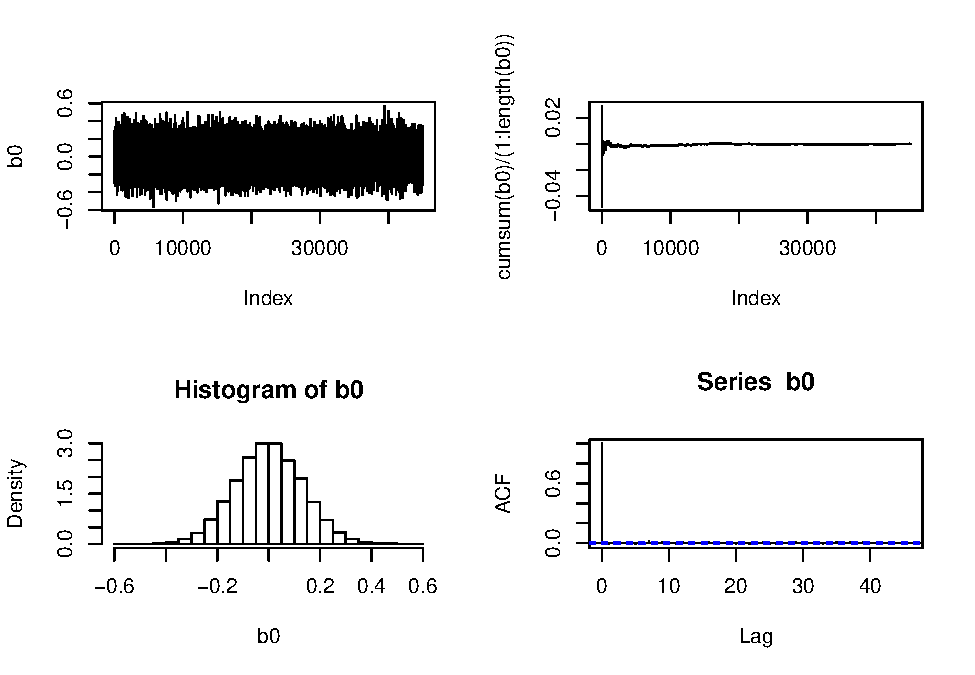
\includegraphics{proyecto_final_nieto_files/figure-latex/unnamed-chunk-3-1.pdf}

\paragraph{Segmentos}\label{segmentos}

Los distintos segmentos con los que contamos y su descripción son los
siguientes:

\textbf{Joven Trabajador} Clientes entre 18 a 34 años,Obreros
calificados,Con ingresos de \$3,300 a \$11,000 mensuales.

\textbf{Joven Profesionista} Clientes entre 18 a 34 años,Joven cuya
profesión requiere una calificación superior para ser desempeñada,Con
ingresos superiores a los \$3,200 mensuales.

\textbf{Pareja Joven} Clientes entre 18 a 34 años,Sin hijos y conviven
en pareja,Con ingresos superiores a los \$5,000 mensuales.

\textbf{Hogares con hijos} Clientes entre 18 a 65 años,Conviven con sus
hijos en el hogar,Con ingresos promedio de \$25,000 mensuales.

\textbf{Pareja Adulta} Clientes entre 35 a 44 años,Sin hijos en el
hogar, que conviven en pareja,Con ingresos superiores a los \$7,000
mensuales.

\textbf{Pareja Senior} Clientes entre 45 a 65 años,Sin hijos en el
hogar, que conviven en pareja,Con ingresos superiores a los \$7,000
mensuales.

\textbf{Divorciado} Clientes entre 35 a 65 años,Divorciados.

\textbf{Adulto Independiente} Clientes entre 35 a 65 años,Sin hijos en
el hogar, ~no conviven en pareja,Con ingresos superiores a ~\$6,000
mensuales.

\textbf{Adulto en Plenitud} Clientes mayores a 65 años.

De forma similar, en la siguiente gráfica se puede observar la serie de
número de créditos contratados por segmento.

\includegraphics{proyecto_final_nieto_files/figure-latex/unnamed-chunk-4-1.pdf}

Y si separamos las tendencias:

\includegraphics{proyecto_final_nieto_files/figure-latex/unnamed-chunk-5-1.pdf}

En la gráfica anterior se muestra que el segmento de hogares con hijos
es el que tiene una tendencia más parecida a la total es decir con más
variaciones en contraste las parejas jóvenes y los divorciados muestran
una tendencia más constante.

Los segmentos con mayor número de contrataciones de forma mensual son
Hogares con Hijos y Adultos en plenitud, y los que menos son Divorciados
y jóvenes trabajadores.

Se presenta una gráfica de caja y brazos donde se notan diferencias
entre los distintos segmentos, como se había mencionado el segmento de
Hogares con hijos es un grupo totalmente separado y el que tiene mayor
volumen de contrataciones, al comparar su rango intercuartílico con
respecto a los demás, por otro lado se puede observar que desde el
segmento de adultos en plenitud hasta jóvenes profesionales al menos el
75\% de los meses han sobrepasado las 40 contrataciones y existe un
tercer grupo donde el volumen y la distribución de contrataciones
mensuales es el el mas bajo, pareja joven, divorciado y joven
trabajador.

\includegraphics{proyecto_final_nieto_files/figure-latex/unnamed-chunk-6-1.pdf}

En la tabla siguiente se observan los estadísticos puntuales de cada
segmento, en esta tabla se puede confirmar lo explicado en la figura 3
de manera puntual, los hogares con hijos es el segmento con mayor número
de contrataciones promedio mensual y también en la mediana de los meses,
después los adultos en plenitud y parejas senior tienen estadísticos
similares y al final los Divorciados y jóvenes trabajadores son los
segmentos con menor número de contrataciones de manera mensual.

\[
\begin{table}[ht]
\centering
\begin{tabular}{rlrr}
  \hline
  & TP\_SEGMENTO\_FINAL2 & mediana & promedio \\ 
  \hline
  1 & HOGARES CON HIJOS & 101.50 & 104.50 \\ 
  2 & ADULTO EN PLENITUD & 68.00 & 67.54 \\ 
  3 & PAREJAS SENIOR & 63.50 & 61.54 \\ 
  4 & ADULTOS INDEPENDIENTES & 55.00 & 54.12 \\ 
  5 & JOVEN PROFESIONAL & 46.00 & 49.79 \\ 
  6 & PAREJAS ADULTAS & 48.00 & 48.62 \\ 
  7 & PAREJA JOVEN & 39.00 & 39.38 \\ 
  8 & DIVORCIADO & 27.50 & 29.17 \\ 
  9 & JOVEN TRABAJADOR & 25.00 & 26.67 \\ 
   \hline
\end{tabular}
\end{table}
\]

\subsection{Modelos Estáticos}\label{modelos-estaticos}

\subsubsection{Modelo lineal normal}\label{modelo-lineal-normal}

\includegraphics{proyecto_final_nieto_files/figure-latex/unnamed-chunk-10-1.pdf}
\includegraphics{proyecto_final_nieto_files/figure-latex/unnamed-chunk-10-2.pdf}
\includegraphics{proyecto_final_nieto_files/figure-latex/unnamed-chunk-10-3.pdf}

DIC:

\begin{verbatim}
## [1] 1634.235
\end{verbatim}

Pseudo-\(R^2\):

\begin{verbatim}
## [1] 0.8373768
\end{verbatim}

\subsubsection{Modelo lineal generalizado poisson con liga
log}\label{modelo-lineal-generalizado-poisson-con-liga-log}

\includegraphics{proyecto_final_nieto_files/figure-latex/unnamed-chunk-14-1.pdf}
\includegraphics{proyecto_final_nieto_files/figure-latex/unnamed-chunk-14-2.pdf}
\includegraphics{proyecto_final_nieto_files/figure-latex/unnamed-chunk-14-3.pdf}

DIC:

\begin{verbatim}
## [1] 1627.145
\end{verbatim}

Pseudo-\(R^2\):

\begin{verbatim}
## [1] 0.8476585
\end{verbatim}

\subsubsection{Modelo lineal generalizado binomial con liga
logística}\label{modelo-lineal-generalizado-binomial-con-liga-logistica}

\includegraphics{proyecto_final_nieto_files/figure-latex/unnamed-chunk-18-1.pdf}
\includegraphics{proyecto_final_nieto_files/figure-latex/unnamed-chunk-18-2.pdf}
\includegraphics{proyecto_final_nieto_files/figure-latex/unnamed-chunk-18-3.pdf}

DIC:

\begin{verbatim}
## [1] 130970760
\end{verbatim}

Pseudo-\(R^2\):

\begin{verbatim}
## [1] 0.8474064
\end{verbatim}


\end{document}
